\documentclass{article}



\usepackage{csquotes}

\usepackage[font=small,labelfont=bf]{caption}
\captionsetup[figure]{font=small}


\usepackage{titlesec}
\titleformat{\section} {\normalfont\fontsize{12}{15}\bfseries}{\thesection}{1em}{}
\titleformat{\subsection} {\normalfont\fontsize{10}{12}\bfseries}{\thesubsection}{1em}{}

% Language setting
% Replace `english' with e.g. `spanish' to change the document language
\usepackage[english]{babel}

% Set page size and margins
% Replace `letterpaper' with `a4paper' for UK/EU standard size
\usepackage[letterpaper,top=2cm,bottom=2cm,left=3cm,right=3cm,marginparwidth=1.75cm]{geometry}

% Useful packages
% \usepackage{mathastext}
\usepackage{amsfonts}
\usepackage{amsmath}
% \usepackage{arevmath}     % For math symbols
\usepackage{graphicx}
\usepackage[colorlinks=true, allcolors=blue]{hyperref}
\usepackage{multicol}
\usepackage{url}
% \usepackage[%  
%     colorlinks=true,
%     pdfborder={0 0 0},
%     linkcolor=blue
% ]{hyperref}

% Chinese Support
\usepackage[CJKmath=true,AutoFakeBold=3,AutoFakeSlant=.2]{xeCJK}   
\setCJKmainfont{NOTOSERIFTC-MEDIUM.OTF}

% Bibtex
\usepackage[
backend=bibtex,
style=numeric,
% sorting=ynt
sorting=none
]{biblatex}
\addbibresource{references/ref.bib}


% Figures
\newenvironment{Figure}
  {\par\medskip\noindent\minipage{\linewidth}}
  {\endminipage\par\medskip}
\usepackage{caption}
\usepackage{wrapfig}
\usepackage{wrapfig}
\usepackage{graphicx}


\title{ICG Final Report}
\author{B10401006 洪愷希, B10502010 王維勤}
\date{}


\begin{document}
\nocite{*}
\setlength{\parindent}{0pt}

\maketitle

\section*{Introduction}
Position based dynamics (PBD) 是一種在圖形領域的新興物理模型框架,由 Matthias M{\"u}ller (2007)等人提出 \cite*{Muller2007-ht}。PBD 並非嚴格意義上的 physics-based simulation,而是一種高效率的近似物理模擬方法,因此主要用於 3D 遊戲等要求效能的場合。PBD 的特點是簡單、穩定、高效,並且容易實現。PBD 的應用範圍廣泛,包括布料模擬、軟體模擬、流體模擬等。本報告將介紹 PBD 的基本原理,並實現布料模擬、軟體模擬等應用。

傳統的物理模擬方法是以力作為核心,即牛頓第二定律:
\begin{align}
  \mathbf{f} = m \mathbf{a}
\end{align}
不過,這也就意味者對於軟體、布料及流體等物體的模擬,需要解決大量的微分方程,計算量極大。相對地,PBD 則是以位置作為核心,即直接修改位置以滿足約束,而不是計算力。這樣的方法不僅簡化了計算,並且可以更容易地處理各種約束,如距離約束、體積約束等。我們將在下一小節中介紹 PBD 的基本原理。

PBD 並不是單一的模型,而是一種框架,因此不乏有許多研究者提出延伸的應用以及改進,例如 position based fluid (PBF) 即是以此框架為基礎進行流體模擬。而在我們的專案中,亦參考了由 PBD 團隊提出的xPBD \cite*{Macklin2016-fh},作為 PBD 的改進版本。

\section*{Position Based Dynamics}
\paragraph{Notations.}
假設我們有 N 個頂點跟 M 個限制條件,對於點 $i \in [1, \cdots , N]$ 有質量 $m_i$、位置 $\mathbf{x}_i$ 以及速度 $\mathbf{v}_i$,
且對一 constraint $j \in [1, \cdots ,M]$ 我們有
\begin{enumerate}
  \item
        A cardinality $n_j$
  \item  A function $C_j: \mathbb{R}^{3n_j} \to \mathbb{R}$.
  \item  A set of indices $\{ i_1, \cdots , i_{n_j} \}, i_k \in [1,N]$.
  \item  A stiffness parameter $k_j \in [0,\cdots ,1]$.
  \item  A type pf either equality or inequality.
\end{enumerate}

\subsection*{Algorithm Overviews}
基於上述之資料以及 time step  $\Delta t$, 這個物體可由\autoref{fig:Alg} 之演算法描述。
在 \autoref{fig:Alg}的演算法中給定的約束 $ C_1, \ldots, C_M $ 在整個模擬過程中固定不變,以下我們對此演算法進行解釋:
在第5行我們考慮外力作用,例如重力,第6行對速度進行 damping。
在第7行,計算外力影響後的新位置 $ \mathbf{p}_i$。
在第9-11行通過 Gauss–Seidel 投影約束並求解。
在第13和14行,移動頂點位置並更新速度。
在第16行則根據摩擦和恢復係數修改碰撞頂點的速度。

\begin{figure}[!ht]
  \centering
  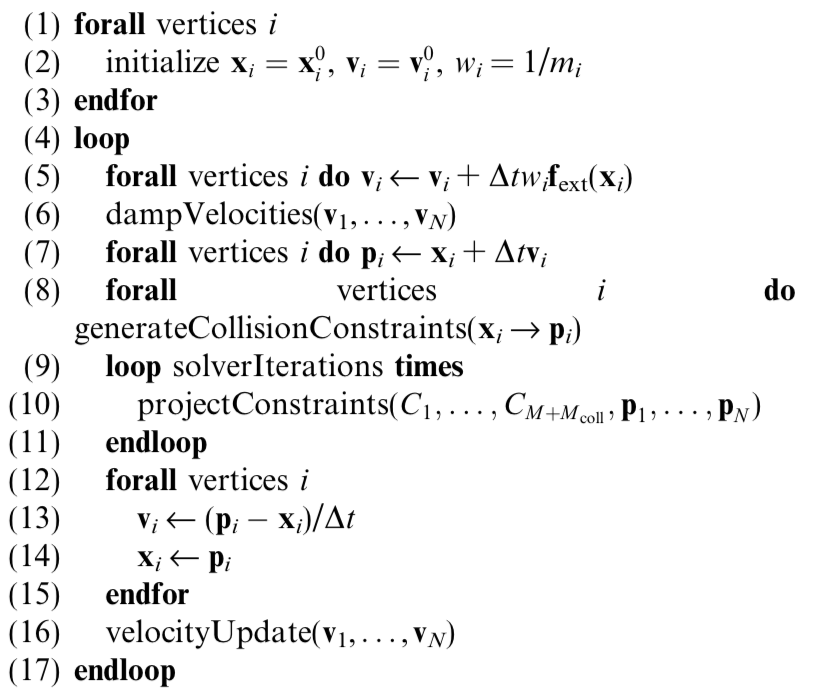
\includegraphics[width=0.5\textwidth]{./figures/alg.png}
  \caption{Algorithm}
  \label{fig:Alg}
\end{figure}


\subsection*{Constraint Projection}
solver  的 input 為 $M + M_{\text{coll}}$ 的 constraints 和每一點的新位置 $\mathbf{p}_1, \ldots, \mathbf{p}_N$。 Solver 將修改這些位置,使其滿足所有 constraints。
我們可發現,即使是一個簡單的距離約束 $C(\mathbf{p}_1, \mathbf{p}_2) = \left|\mathbf{p}_1 - \mathbf{p}_2\right| - d$ 也會產生非線性方程。

為了解決這樣一組方程和不等式,我們使用類似於 Gauss-Seidel 的方法,逐一獨立解決每個約束。

我們藉由移動這些點以滿足該 constraint。過程中需滿足動量以及角動量的守恆。
令 $\Delta p_i$ 為 the displacement of vertex i by the projection.
考慮動量守恆
\begin{align}
  \sum_i m_i \Delta \mathbf{p}_i = 0,
\end{align}

考慮角動量守恆
\begin{align}
  \sum_i \mathbf{p}_i \times \Delta \mathbf{p}_i = 0.
\end{align}

如果投影違反了以上限制,將會產生 ghost force,如同外力一般拖動和旋轉物體。
令 $\mathbf{p} = \left[ \mathbf{p}^\top_1 \cdots \mathbf{p}^\top_n  \right] $。
可以發現當 $\Delta \mathbf{p}$ 在 $\nabla_p C(\mathbf{p})$ 的方向且每一點質量皆相同時,動量守恆成立。
考慮內部約束,對於 $\mathbf{p}$,我們想求得 correction 以滿足 $ C(\mathbf{p}+ \Delta \mathbf{p}) = 0$。
此關係式可以寫成
\begin{align}
  C(\mathbf{p}+ \Delta \mathbf{p}) \approx C(\mathbf{p}) + \nabla_p C(\mathbf{p}) \cdot \Delta \mathbf{p} = 0
\end{align}

我們限制 $\Delta \mathbf{p}$ 在 $\nabla_p C(\mathbf{p})$ 的方向,意即
\begin{align}
  \Delta \mathbf{p} = \lambda \nabla_p C(\mathbf{p})
\end{align}
\begin{align}
  \Delta \mathbf{p} = - \frac{C(\mathbf{p})}{\left|\nabla_p C(\mathbf{p})\right|^2}  \nabla_p C(\mathbf{p}).
\end{align}

對於 individual point $\mathbf{p}_i$ 的  correction,我們有
\begin{align}
  \Delta \mathbf{p}_i = -s \nabla_{\mathbf{p}_i} C(\mathbf{p}_1, \cdots , \mathbf{p}_n)
\end{align}
而對於每一點,scaling factor 皆為
\begin{align}
  s = \frac{C(\mathbf{p}_1 , \cdots , \mathbf{p}_n) }{\sum_j \left|\nabla_{p_j}  C(\mathbf{p}_1 , \cdots , \mathbf{p}_n) \right|^2 }
\end{align}

對於每一點質量不一定相同之情況,我們令 $w_i = 1 / m_i$ 於是
\begin{align}
  \Delta \mathbf{p}_i = -s \frac{n \cdot w_i}{\sum_j w_j} \nabla_{p_i} C(\mathbf{p}_1 , \cdots , \mathbf{p}_n),
\end{align}
舉例來說,我們考慮下列 constraint
\begin{align}
  C ( \mathbf{p}_1 , \mathbf{p}_2) = \left|\mathbf{p}_1 - \mathbf{p}_2\right| -d
\end{align}
其微分為
\begin{align}
  \nabla_{p_1} C(\mathbf{p}_1 , \mathbf{p}_2) & = n  \\
  \nabla_{p_2} C(\mathbf{p}_1 , \mathbf{p}_2) & = -n
\end{align}
其 final corrections 為
\begin{align}
  \Delta \mathbf{p}_1 & = - \frac{w_1}{w_1+ w_2} \left( \left|\mathbf{p}_1 - \mathbf{p}_2\right| -d \right) \frac{\mathbf{p}_1 - \mathbf{p}_2}{\left|\mathbf{p}_1 - \mathbf{p}_2\right|} \\
  \Delta \mathbf{p}_2 & = - \frac{w_2}{w_1+ w_2} \left( \left|\mathbf{p}_1 - \mathbf{p}_2\right| -d \right) \frac{\mathbf{p}_1 - \mathbf{p}_2}{\left|\mathbf{p}_1 - \mathbf{p}_2\right|}
\end{align}

\section*{Soft Body Simulation}

現在考慮 soft body simulation。將模型以 mesh 的方式建構,可以將它視為多個 tetrahedral 所組成的 3D 結構。為了維持模型的穩定,針對各個 tetrahedral 以及其vertex,考慮以下兩個 constraints:distance constraint, volume constraint。

\subsection*{Distance Constraint}
針對 distance constraint,考慮mesh中任兩點$\mathbf{x}_1$, $\mathbf{x}_2$距離$l = \left|\mathbf{x}_1 - \mathbf{x}_2\right|$不變,設定 constraint 為
\begin{align}
  C = l - l_0 \label{eq:Dis}
\end{align}

\begin{figure}[!ht]
  \centering
  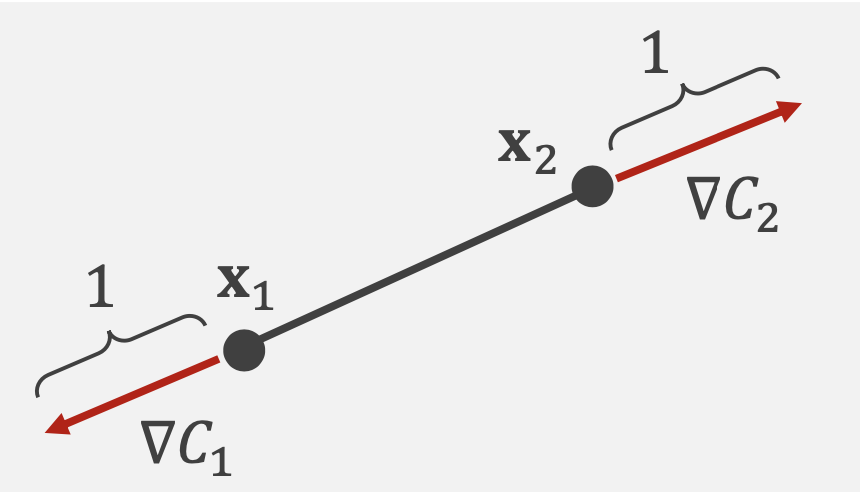
\includegraphics[width=0.5\textwidth]{./figures/distanceConstraint.png}
  \caption{Distance Constraint}
  \label{fig:Dis}
\end{figure}

而 gradient 即延兩點連線方向,大小為 1
\begin{align}
  \nabla C_1 = \frac{\mathbf{x}_1 - \mathbf{x}_2}{\left|\mathbf{x}_1 - \mathbf{x}_2\right|} \\
  \nabla C_2 = \frac{\mathbf{x}_2 - \mathbf{x}_1}{\left|\mathbf{x}_2 - \mathbf{x}_1\right|} \\
  \lambda = \frac{-(l-l_0)}{w_1\cdot 1 + w_2 \cdot 1}
\end{align}

更新位置為
\begin{align}
  \Delta \mathbf{x}_1 = \lambda w_1 \nabla C_1
  = - \frac{w_1}{w_1 + w_2} (l - l_0) \frac{\mathbf{x}_2 - \mathbf{x}_1}{\left|\mathbf{x}_2 - \mathbf{x}_1\right|}
\end{align}

\subsection*{Volume Constraint}
針對 tetrahedral,為保持體積不變,我們設定其 volume constraint 為
\begin{align}
  C = 6(V - V_0)
\end{align}

考慮 constraint 的 gradient 方向為體積變化最大方向即垂直底面方向,如\autoref{fig:Vol}所示,以底邊外積來計算可以有以下結果
\begin{align}
  \nabla_1 C & = (\mathbf{x}_4 - \mathbf{x}_1) \times (\mathbf{x}_3 - \mathbf{x}_2) \\
  \nabla_2 C & = (\mathbf{x}_3 - \mathbf{x}_1) \times (\mathbf{x}_4 - \mathbf{x}_1) \\
  \nabla_3 C & = (\mathbf{x}_4 - \mathbf{x}_1) \times (\mathbf{x}_2 - \mathbf{x}_1) \\
  \nabla_4 C & = (\mathbf{x}_2 - \mathbf{x}_1) \times (\mathbf{x}_3 - \mathbf{x}_1)
\end{align}

\begin{figure}[!ht]
  \centering
  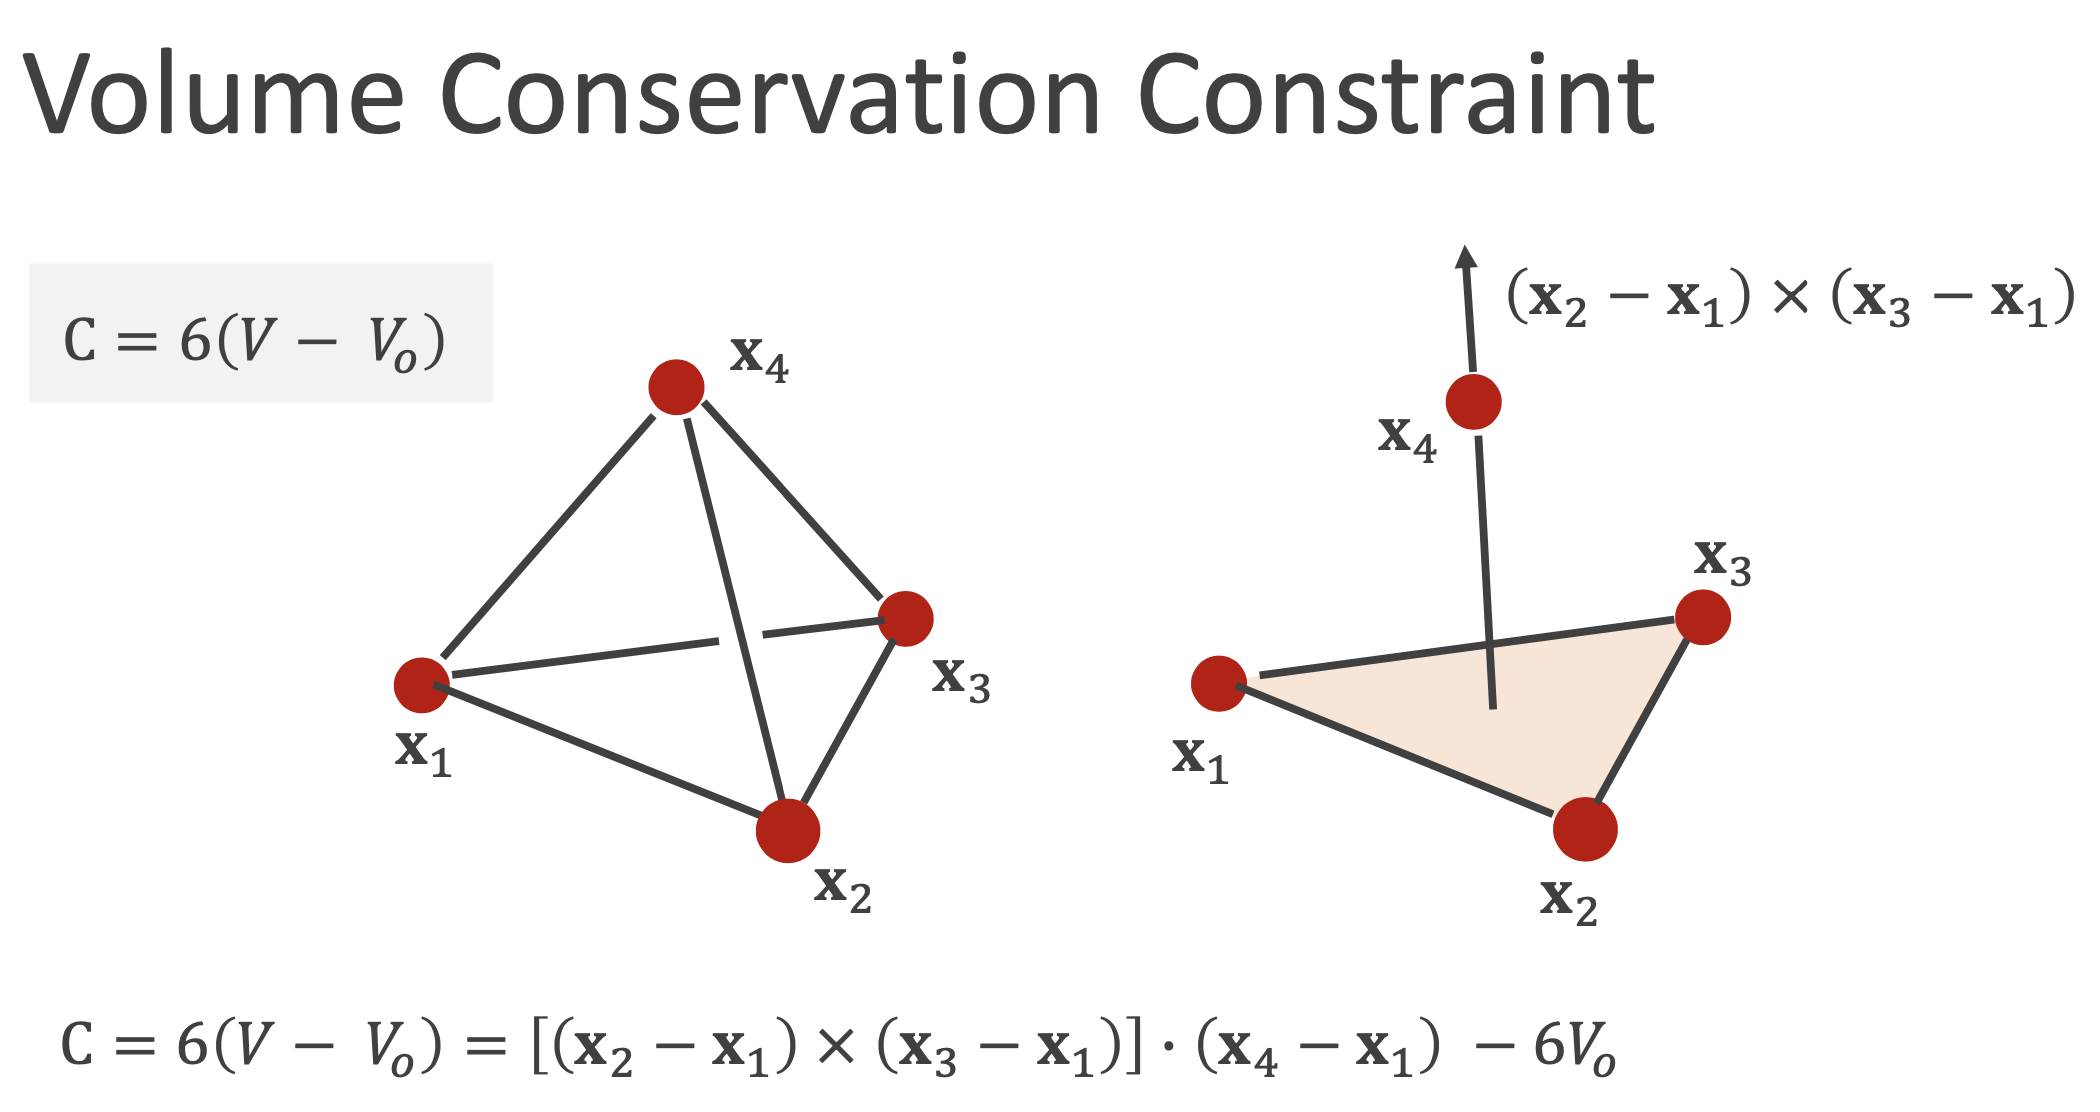
\includegraphics[width=0.5\textwidth]{./figures/volumeConstraint.png}
  \caption{Volume Constraint}
  \label{fig:Vol}
\end{figure}

\begin{align}
  \lambda = \frac{-6(V - V_0)}{w_1\left|\nabla C_1\right|^2 + w_2\left|\nabla C_2\right|^2 + w_3\left|\nabla C_3\right|^2 + w_4\left|\nabla C_4\right|^2 + \frac{\alpha}{\Delta t ^ 2}}
\end{align}

最終更新位置
\begin{align}
  \Delta \mathbf{x}_i = \lambda w_i \nabla C_i
\end{align}

\section*{Cloth Simulation}

\subsection*{Bending Constraint}

對於布料的模擬,我們使用了兩種 constraint:distance constraint 和 bending constraint。
Distance constraint 用於保持同一個三角形上的點之間的距離,而 bending constraint 用於保持相鄰三角形的角度。由於 distance constraint 已經在 soft body simulation 中介紹過,這裡我們將重點放在 bending constraint 上。

在 \autoref{fig:bending} 中,兩個相鄰三角形的頂點為 $\mathbf{p_1}, \mathbf{p_2}, \mathbf{p_3}, \mathbf{p_4}$。則兩個面的法向量分別為
\begin{align}
  \mathbf{n_1} & = \frac{(\mathbf{p_2}-\mathbf{p_1})\times(\mathbf{p_3}-\mathbf{p_1})}{|(\mathbf{p_2}-\mathbf{p_1})\times(\mathbf{p_3}-\mathbf{p_1})|} \\
  \mathbf{n_2} & = \frac{(\mathbf{p_2}-\mathbf{p_1})\times(\mathbf{p_4}-\mathbf{p_1})}{|(\mathbf{p_2}-\mathbf{p_1})\times(\mathbf{p_4}-\mathbf{p_1})|}
\end{align}
因此對於兩者夾角的 constraint 可表示為
\[
C_{bend}( \mathbf{p_1}, \mathbf{p_2}, \mathbf{p_3}, \mathbf{p_4}) = \arccos{\mathbf{n_1} \cdot \mathbf{n_2}} - \phi_0
\]
其中 $\phi_0$ 為初始角度。

\begin{figure}[!ht]
  \centering
  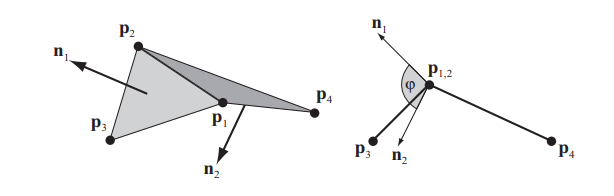
\includegraphics[width=0.6\linewidth]{figures/bending.png}
  \caption{Bending constrint 示意圖}
  \label{fig:bending}
\end{figure}

\section*{Collision}

對於物體之間的碰撞,我們使用 distance constraint 來處理。當兩個質點的距離小於一定值時,我們施加 \ref*{eq:Dis} 中的 constraint,並且令 $l_0$ 為事先訂好的參數。如此一來在 constraint solver 中即可處理碰撞問題。

若是對每兩個質點都判斷是否碰撞,計算量將會過大。因此我們使用 spatial hashing 的技巧,將空間分成一個個的格子,並且將每個質點放入對應的格子中。這樣一來,我們只需要對每個格子中的質點進行碰撞判斷,大大減少了計算量。

\section*{Results}

我們以每個 step 有 10 個 substep 進行模擬,畫面中約有 6000 個三角形。

\begin{figure}[!ht]
  \centering
  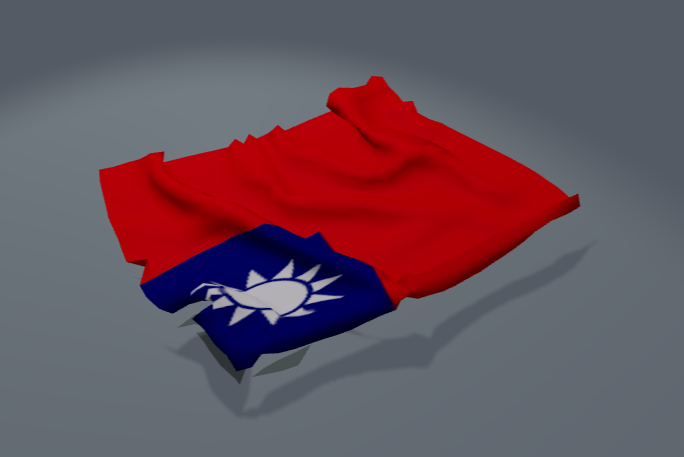
\includegraphics[width=0.6\linewidth]{figures/flag1.png}
  \caption{模擬布料掉落地面,可見有褶皺的現象}
\end{figure}

\begin{figure}[!ht]
  \centering
  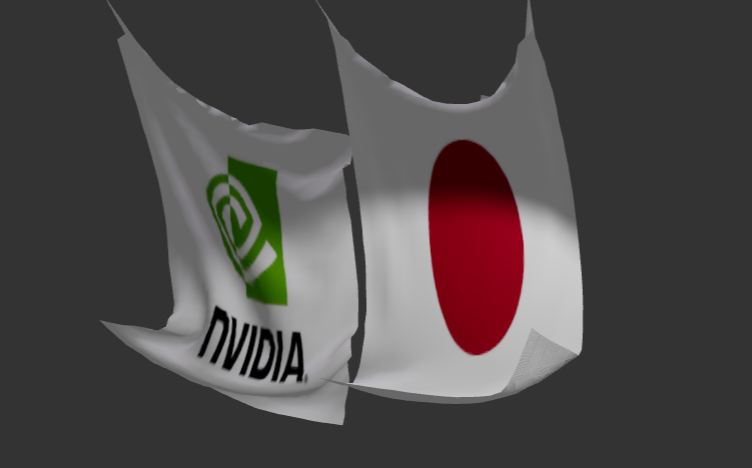
\includegraphics[width=0.6\linewidth]{figures/flag2.png}
  \caption{模擬布料懸掛空中,並加上水平的風力}
\end{figure}

\begin{figure}[!ht]
  \centering
  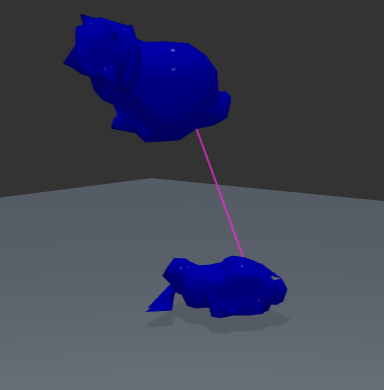
\includegraphics[width=0.6\linewidth]{figures/bunny.png}
  \caption{以兔子模型模擬 soft body。另外在兩個兔子間加上距離的 constraint}
\end{figure}

\begin{figure}[!ht]
  \centering
  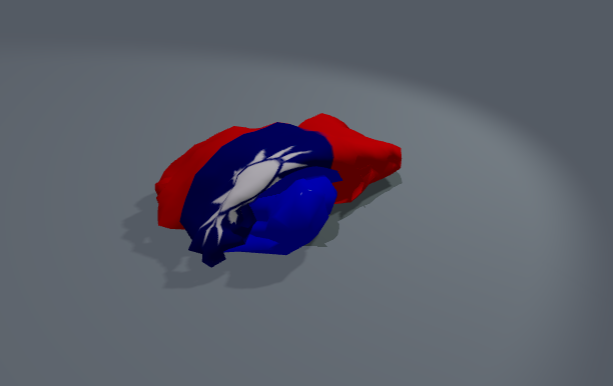
\includegraphics[width=0.6\linewidth]{figures/collision.png}
  \caption{布料與兔子間的碰撞}
\end{figure}


\begin{figure}[!ht]
  \centering
  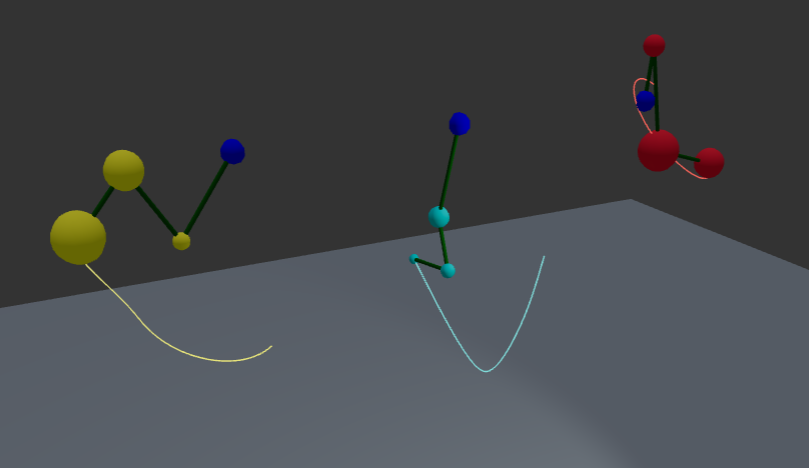
\includegraphics[width=0.6\linewidth]{figures/pendulums.png}
  \caption{模擬多重單擺串接,起始畫面}
\end{figure}


\begin{figure}[!ht]
  \centering
  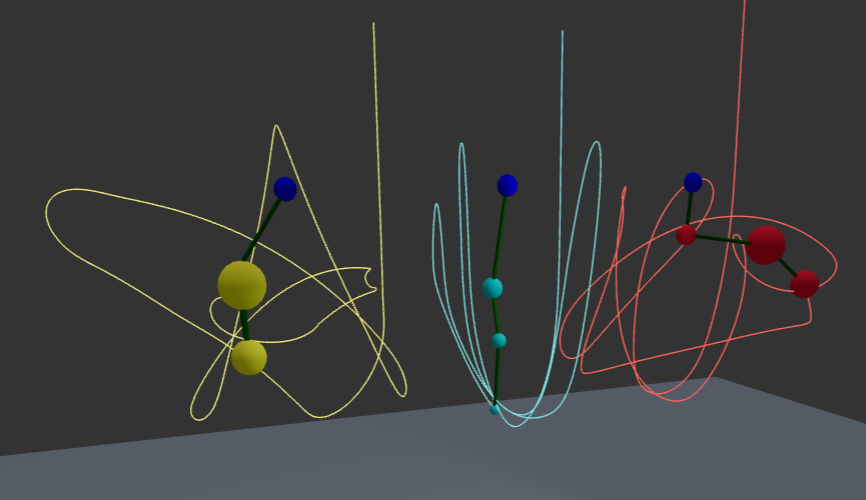
\includegraphics[width=0.6\linewidth]{figures/pendulums1.png}
  \caption{模擬多重單擺串接,運行數秒後之軌跡}
\end{figure}



\clearpage
\printbibliography[title={}]

\end{document}
